%%%%%%%%%%%%%%%%%%%%%%% file template.tex %%%%%%%%%%%%%%%%%%%%%%%%%
%
% This is a general template file for the LaTeX package SVJour3
% for Springer journals.          Springer Heidelberg 2010/09/16
%
% Copy it to a new file with a new name and use it as the basis
% for your article. Delete % signs as needed.
%
% This template includes a few options for different layouts and
% content for various journals. Please consult a previous issue of
% your journal as needed.
%
%%%%%%%%%%%%%%%%%%%%%%%%%%%%%%%%%%%%%%%%%%%%%%%%%%%%%%%%%%%%%%%%%%%
%
% First comes an example EPS file -- just ignore it and
% proceed on the \documentclass line
% your LaTeX will extract the file if required
\begin{filecontents*}{example.eps}
%!PS-Adobe-3.0 EPSF-3.0
%%BoundingBox: 19 19 221 221
%%CreationDate: Mon Sep 29 1997
%%Creator: programmed by hand (JK)
%%EndComments
gsave
newpath
  20 20 moveto
  20 220 lineto
  220 220 lineto
  220 20 lineto
closepath
2 setlinewidth
gsave
  .4 setgray fill
grestore
stroke
grestore
\end{filecontents*}
%
\RequirePackage{fix-cm}
%
%\documentclass{svjour3}                     % onecolumn (standard format)
%\documentclass[smallcondensed]{svjour3}     % onecolumn (ditto)
%\documentclass[smallextended]{svjour3}       % onecolumn (second format)
\documentclass[twocolumn]{svjour3}          % twocolumn
%
\smartqed  % flush right qed marks, e.g. at end of proof
%
\usepackage{graphicx}
\usepackage[table,xcdraw]{xcolor}
\graphicspath{ {./images/}{./images/created}{./images/generation} }
%
% \usepackage{mathptmx}      % use Times fonts if available on your TeX system
%
% insert here the call for the packages your document requires
%\usepackage{latexsym}
% etc.
%
% please place your own definitions here and don't use \def but
% \newcommand{}{}
%
% Insert the name of "your journal" with
% \journalname{myjournal}
%
\begin{document}

\title{Malaria Blood Smears Object Detection using DCGAN Networks}
%\subtitle{Do you have a subtitle?\\ If so, write it here}

%\titlerunning{Short form of title}        % if too long for running head

\author{Francisco Nauber Bernardo Gois         \and
        João Alexandre Lôbo Marques \and
        Márcio Costa Santos   \and
        Allberson Bruno de Oliveira Dantas \and 
        Simon James Fong
        %etc.
}

%\authorrunning{Short form of author list} % if too long for running head

\institute{Nauber Gois \at
              Universidade Federal de Fortaleza \\
              Tel.: +123-45-678910\\
              Fax: +123-45-678910\\
              \email{naubergois@ufc.br}           %  \\
%             \emph{Present address:} of F. Author  %  if needed
           \and
           Joao Alexandre Lobo Marques \at
           University of Saint Joseph (Macao) \\
           \and
           Marcio Costa Santos \\
           Universidade Federal de Fortaleza \\
}



\date{Received: date / Accepted: date}
% The correct dates will be entered by the editor


\maketitle

\begin{abstract}
Fast and efficient diagnosis of malaria cases is essential in efforts to eliminate the disease. The default to diagnose malaria is a microscopy exam. This process becomes problematic when cases happen in rural areas and experts cannot be present to make such a diagnosis. Automation of the diagnostical process with the use of an intelligent system that would recognize malaria parasites could aid in problem resolution. Several laboratories capture the images in low quality using a system of microscopes based on mobile devices. Due to the poor quality of this system, conventional algorithms do not process these images pro- perly. The use of Deep Learning may be a way to improve the accuracy of the present method. nevertheless, such an approach usually requires a large number of training sets, which is the reason why is difficult to apply to diagnostic systems deep learning techniques, since the data are usually protected by medical confi- dentiality. The use of Generating Adverse Networks can help in generating data for training and improving the accuracy of deep learning models. The objective of this research project is to use Generating Adversarial Networks in conjunc- tion with deep learning models in order to improve accuracy in the diagnosis of malaria in peripheral blood smears.
\keywords{Malaria  \and Generative Adversarial Network \and More}
% \PACS{PACS code1 \and PACS code2 \and more}
% \subclass{MSC code1 \and MSC code2 \and more}
\end{abstract}

\section{Introduction}
\label{intro}


The global burden of malaria is enormous. In 2012, the World Health Organization (WHO) estimated at least 247 million of worldwide people suffer from malaria and more than two billion or 42\% of of worldwide people has a risk of malaria because of living in malaria endemic areas, 627,000 of which resulted in deaths among African children. In the Philippines, malaria is considered to be the 9th leading cause of morbidity, with 58 out of the 81 provinces being malaria-endemic. Among the major obstacles for malaria eradication are the remote location of the majority of malaria cases and the lack of trained individuals that can analyze blood samples using
microscopy. The gold standard test for malaria is the method of preparing a blood smear on a glass slide, staining it, and examining it under a microscope. While several rapid diagnostic tests are also currently available, they still have shortcomings compared to microscopical analysis \cite{Quinn2016DeepDiagnostics}\cite{Premaratne2006AFilms}\cite{Penas2017}.


This is where automated systems for diagnosis
come in. Instead of manually going over a blood sample and
checking for the presence of malaria parasites, photographs
of the sample viewed from the microscope are analyzed by
an intelligent system. With such systems, the remote location
of malaria cases becomes less of a problem if such systems
become publicly available as trained microscopists and doctors \cite{Premaratne2006AFilms}\cite{Penas2017}.

Malaria is a disease caused by protozoa parasite of the genus Plasmodium that infects erythrocytes of patients. The one of Plasmodium species that infect humans is Plasmodium falciparum. This species is the most virulent because in a short time can invades erythrocytes in large numbers. Moreover, it causes various complications in the body's organs, and even causes the death. Most of these deaths were caused by the Plasmodium falciparum that infects red blood cells of patients which is characterized by a variety of organ dysfunction \cite{Dong2017}.


Malaria rapid diagnostic tests (RDTs) are relatively simple to perform and provide results quickly for making treatment decisions. However, the accuracy and application of RDT
results depends on several factors such as quality of the RDT, storage, transport and end user performance. A cross sectional survey to explore factors that affect the performance and use of
RDTs was conducted in the primary care facilities in South Africa \cite{Moonasar2007}


In the last decade, deep learning  methods have shown successful outcomes in different applications, including signal processing, object recognition, natural language processing, etc. Their attraction comes from the automatic feature learning ability in a deep network architecture 

Our objective was to develop an automated tool recognition of intracellular malaria parasites in stained blood films.   

\section{Convolutional Neural Networks}

\section{Generative Adversarial Networks}

Learning reusable resource representations from large datasets has been an active research area. One way to build good image representations is through Generative Adversarial Networks. Generator Adverse Networks (GAN) learn to synthesize elements of a target distribution using two competing neural networks. GAN networks can produce compelling images that are sharper than those produced by automatic encoders using pixel losses. The Generator (G) network selects an n-dimensional random sample from a predefined distribution, conventionally called latent space and attempts to create examples of the target distribution. The discriminant network (D) takes a generated or real example as input and has to make the binary decision whether the input is real or generated. This competition process is expressed as a zero-sum game in the following loss term:

Let x be a natural image taken from a distribution, $ p_X$ and be a random vector \textit{z} in $ {\rm I\!R}^d $. Considering that z is of a uniform distribution with the support $[1-1]^d$, then \textit{g} and \textit{f} are the generator and discriminative models, respectively. Denoting the distribution \textit{g(z)} to $ p_G $. The discriminative model estimates the probability that an input image was generated by $ p_X $. Ideally, \textit{f(x)=1}  if $x  \sim\  p_X$ and \textit{f (x) = 0} if $ x \sim\ p_G $. A generator network corresponds to a mini-game with two players, the generator and discriminative models, trained according to the equation \cite{Liu2016}:


\begin{equation}
\medmath{ \underset{g}{max} \underset{f}{min} V(f,g)= \mathbb{E}_{x \sim px} [-log(f(x))]+\mathbb{E}_{z \sim pz}[-log(1-f(g(z)))]} 
\end{equation}


The equation is solved by applying the gradient in two steps:

\begin{equation}
\theta^{t+1}_{f} = \theta^{t}_{f} -\lambda^t \nabla_{\theta f} V (f^t, g^t)
\end{equation}

\begin{equation}
\theta^{t+1}_{g} = \theta^{t}_{g} -\lambda^t \nabla_{\theta g} V (f^t+1, g^t)
\end{equation}


$ \theta_f $ and $ \theta_g $ are parameters of f and g, $ \ lambda $ is the learning rate and t is the number of iterations.

Goodfellow et al. show that given sufficient capacity for f and g training iterations, the distribution $ p_G $ converges to $ p_X $. In other words, from a random vector z, the network g can synthesize an image g (z) that resembles one that is extracted from the true distribution $ p_X $. \cite{Goodfellow2014}.

Building a good generative model of natural images has been a fundamental problem. However, images are complex and high dimensional, making them hard to model well. Generative Adversarial Networks \cite{Goodfellow2014} generated images suffering from being noisy and incomprehensible. A laplacian pyramid extension to this approach showed higher quality images, but they still suffered from the objects looking wobbly because of noise introduced in chaining multiple models \cite{Denton2015}. A recurrent network approach \cite{gregor2015draw} and a deconvolution network approach (Dosovitskiy et al., 2014) have also recently had some success with generating natural images. However, they have not leveraged the generators for supervised tasks.

Radford et al.  introduce a new class of CNNs called deep convolutional generative adversarial networks (DCGANs) \cite{Radford2015UnsupervisedNetworks}. The main differences of DCGANS are: Convert max-pooling layers to convolution layers; Convert fully connected layers to global average pooling layers in the discriminator; Use batch normalization layers in the generator and the discriminator and use leaky ReLU activation functions in the discriminator.

\section{Deep Learning for Malaria Diagnosis}

In this project, a preliminary systematic mapping of the state of the art was conducted based on the process described by Petersen et al. \cite{Petersen2015} according to which, there are five essential steps to be followed: (i) definition of research questions, (ii) conducting research on relevant primary studies, (iii) document screening, (iv) extract keywords of abstracts, and (v) data extraction and mapping. Considering that research questions should exemplify the objectives of the mapping study, the following question was elaborated: Which research from 2002 to 2018 applied the use of deep learning in the diagnosis of malaria using peripheral blood smears?

Initially searches were performed with keywords consisted of the combination of the word Malaria, machine learning, deep learning and synonyms. In the first step, all primary studies retrieved were evaluated in order to identify those relevant to answer the research questions. After reading the titles, abstracts and keywords, this initial set was reduced to 16 articles that contained studies related to the use of deep learning.

Rajpurkar et al. have developed a reinforcement learning agent (RL) that can predict the probability of an individual positive test for malaria by asking questions about your home. After the learning phase, the agent determines the next question in the survey and uses stopping criteria to forecast malaria probability based on your responses so far \cite{Rajpurkar2017}. Gueorguieva et al. applied the Faster R-CNN object detection model to identify cells and recognize their stages in clear field microscopy images of malaria-infected blood \cite{hung2017applying}. Poostchi et al. presents a systematic review with a set of approaches for malaria automatic diagnosis \cite{Poostchi2018}.


Zhang et al. presented a two-step approach to detecting infected and uninfected cells. The first step applies an object-detection structure with trained classifier to detect all red blood cells in a blood drop image. The second stage classifies each segmented region into an infected or uninfected cell, applying morphological characteristics \cite{Zhang2016}. Liang et al. use a convolutional neural network to discriminate between infected and uninfected cells in fine blood smears after the application of a conventional cell segmentation approach classification \cite{Liang2017}.

Other authors who have applied deep learning in cell segmentation are Dong et al. and Gopakumar et al. who used convolutional neural networks. Dong et al. used whole images of thin blood slides to compile a dataset of red blood cells infected with malaria and uninfected cells as labeled by a group of four pathologists. Three types of known convolutional neural networks were evaluated, including LeNet, AlexNet and GoogLeNet. The simulation results showed that all these deep convolution neural networks achieved classification accuracies of more than 95 \%, greater than the accuracy of about 92 \% achievable using the support vector machine (SVM) method. In addition, deep learning methods have the advantage of being able to automatically learn the characteristics of the incoming data, thus requiring the least amount of human expert inputs for automated malaria diagnosis \cite {Dong2017} \cite{Dong2017a}. Bibin et al. used deep belief networks, and recently Hung et al. presented an end-to-end structure using faster convolutional neural network.

Premaratne et al. used digital images of oil immersion views from microscopic slides captured though a capture card. They were preprocessed by segmentation and grayscale conversion to reduce their dimensionality and later fed into a feed forward backpropagation neural network (NN) for training \cite{Premaratne2006AFilms}.

Among the studies investigated, the use of Generative Adversarial Networks for the generation of new samples of peripheral blood smears was not presented. The present research intends to use Generating Adversarial Networks to generate new samples of peripheral blood smears with the objective of improving the accuracy in automatic diagnosis in cases of malaria.





\section{The Proposed Method -GAN network object detection method}
\label{segmethod}

In this section, we describe the process for object detection in using GAN network object detection method. The process consist of the following steps: blood smears image acquisition, image generation with GANs networks (Figure \ref{fig:maincomp} -\ding{202} ); train a convolutional neural network (Figure \ref{fig:maincomp} -\ding{203});  apply adaptive  threshold filter (Figure \ref{fig:maincomp} -\ding{204}) and classify objects with the trained convolutional network (Figure \ref{fig:maincomp} -\ding{205}). 

Several experiments where conducted in order to analyse the benefits of use GAN networks in the proposed method. The images for the experiments where acquired from the repository presented by Quinn et al. \cite{Quinn2016DeepDiagnostics}.  The code are developed in python language using the Keras framework.

The experiments used a Deep convolutional generative adversarial network according to the architecture shown in figure


\lstset{basicstyle=\footnotesize\ttfamily,breaklines=true}
\begin{lstlisting}[language=Python,numbers=left,frame=tb,caption=Generator Keras Code]
model = Sequential()

model.add(Dense(512 * 7* 7, activation="relu",     
input_dim=self.latent_dim))

model.add(Reshape((7,7, 512)))
model.add(UpSampling2D())
model.add(Conv2D(256, kernel_size=3, padding="same"))
model.add(BatchNormalization(momentum=0.8))
model.add(Activation("relu"))
model.add(UpSampling2D())
model.add(Conv2D(128, kernel_size=3, padding="same"))
model.add(BatchNormalization(momentum=0.8))
model.add(Activation("relu"))
model.add(UpSampling2D())
model.add(Conv2D(64, kernel_size=3, padding="same"))
model.add(BatchNormalization(momentum=0.8))
model.add(Activation("relu"))
model.add(UpSampling2D())
model.add(Conv2D(32, kernel_size=3, padding="same"))
model.add(BatchNormalization(momentum=0.8))
model.add(Activation("relu"))
model.add(Conv2D(self.channels, 
            kernel_size=3, padding="same"))
model.add(Activation("tanh"))

model.summary()

noise = Input(shape=(self.latent_dim,))
img = model(noise)

\end{lstlisting}


\begin{figure*}[h]
\caption{Main components of the proposed method .}
\label{fig:maincomp}
  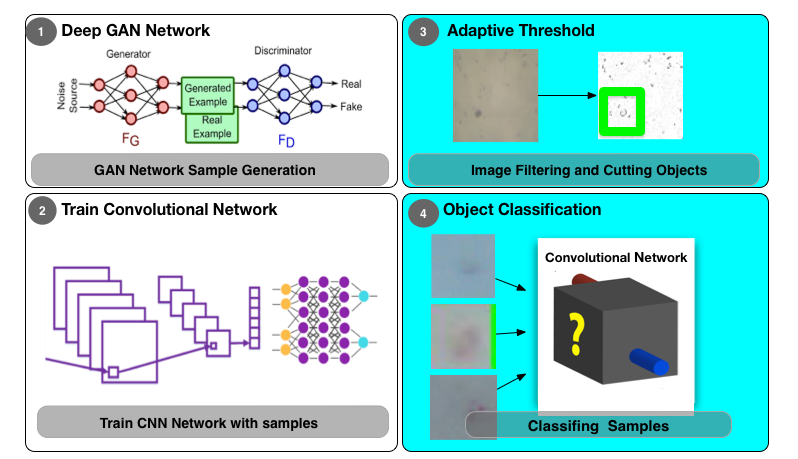
\includegraphics[width=\textwidth]{images/MainComponents.png}
  
\end{figure*}



\begin{figure}[h]
\caption{Main components of the proposed method .}
\label{fig:gen50}
\begin{center}
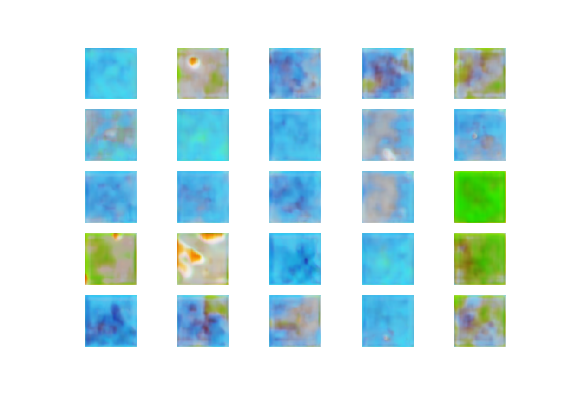
\includegraphics[scale=0.45]{./images/generation/alta_mnist_50.png} \end{center}\caption{Generated images after 50 epochs}
\end{figure}

\begin{figure}[h]
\caption{Generated images after 250 epochs}
\label{fig:gen250}
\begin{center}
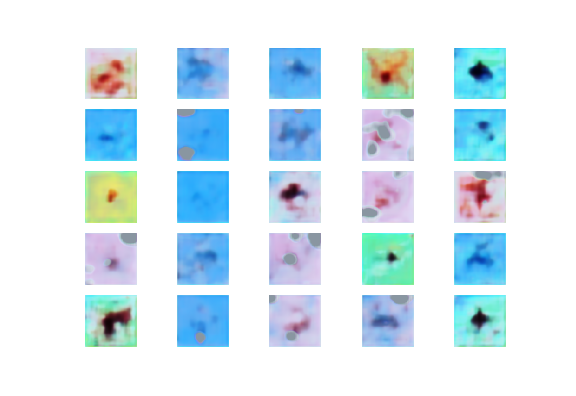
\includegraphics[scale=0.45]{./images/generation/alta_mnist_250.png} \end{center}

\end{figure}


\begin{figure}[h]
\label{fig:gen30410}
\begin{center}
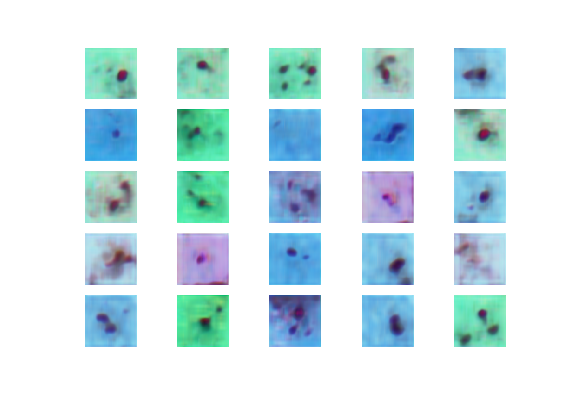
\includegraphics[scale=0.45]{./images/generation/alta_mnist_30410.png} \end{center}
\caption{Generated images after 30410 epochs}
\end{figure}



\begin{figure*}[htp]
  \centering
  \subfigure[random caption 1]{
  %\caption{Generated images after 30410 epochs}
  %\label{fig:threshold}
  
\includegraphics[scale=0.21]{./images/threshold.png}
  }
  \subfigure[random caption 2]{
  %\caption{Generated images after 30410 epochs}
  %\label{fig:objectdetect}
  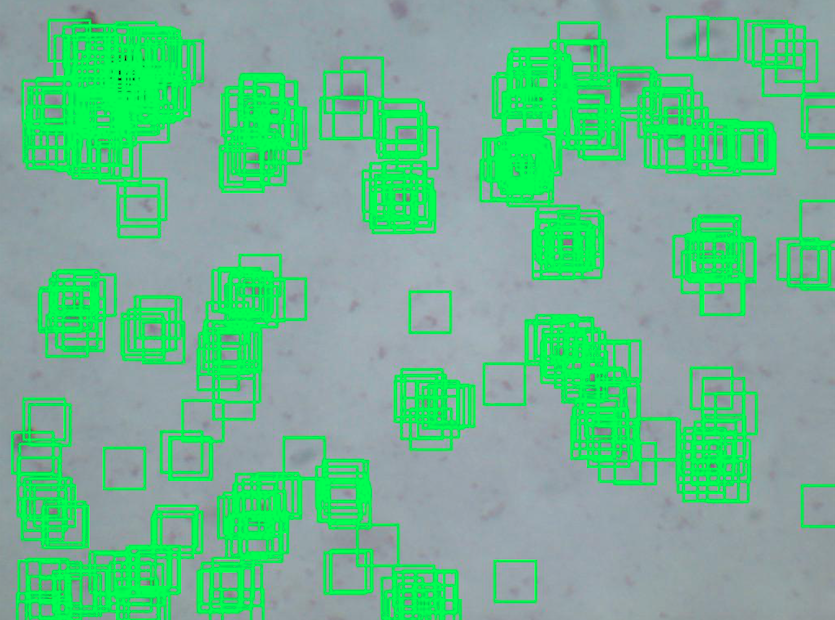
\includegraphics[scale=0.25]{./images/object_detected.png}
  }
\end{figure*}


% Please add the following required packages to your document preamble:
% \usepackage[table,xcdraw]{xcolor}
% If you use beamer only pass "xcolor=table" option, i.e. \documentclass[xcolor=table]{beamer}
\begin{table}[h]
\caption{Results of training the CNN network with images generates by DGAN network}
\label{tab:results}
\begin{tabular}{|l|l|l|l|}
\hline
\rowcolor[HTML]{C0C0C0} 
\textbf{\begin{tabular}[c]{@{}l@{}}Number of \\ Samples \\ Created\\ by GAN \\ Network\end{tabular}} & \textbf{\begin{tabular}[c]{@{}l@{}}Number of\\ Real \\ Images\\ for Test\end{tabular}} & \textbf{\begin{tabular}[c]{@{}l@{}}Number \\ of correctly \\ classified \\ samples\end{tabular}} & \textbf{\begin{tabular}[c]{@{}l@{}}Number of \\ incorrectly \\ classified \\ samples\end{tabular}} \\ \hline
600                                                                                            & 600                                                                                 & 420 (70 \%)                                                                                      & 180                                                                                                \\ \hline
800                                                                                            & 600                                                                                 & 406 (68 \%)                                                                                      & 194                                                                                                \\ \hline
1000                                                                                           & 600                                                                                 & 453 (76 \%)                                                                                      & 147                                                                                                \\ \hline
1200                                                                                           & 600                                                                                 & 424 (71 \%)                                                                                      & 176                                                                                                \\ \hline
1400                                                                                           & 600                                                                                 & \begin{tabular}[c]{@{}l@{}}429 \\ ($\sim$71 \%)\end{tabular}                                     & 171                                                                                                \\ \hline
1600                                                                                           & 600                                                                                 & 430 (72 \%)                                                                                      & 170                                                                                                \\ \hline
1800                                                                                           & 600                                                                                 & 480 (80  \%)                                                                                     & 120                                                                                                \\ \hline
2200                                                                                           & 600                                                                                 & 600 (100 \%)                                                                                     & 0                                                                                                  \\ \hline
\end{tabular}
\end{table}



\section{Conclusion}


%\begin{acknowledgements}
%If you'd like to thank anyone, place your comments here
%and remove the percent signs.
%\end{acknowledgements}

% BibTeX users please use one of
%\bibliographystyle{spbasic}      % basic style, author-year citations
%\bibliographystyle{spmpsci}      % mathematics and physical sciences
%\bibliographystyle{spphys}       % APS-like style for physics
%\bibliography{}   % name your BibTeX data base

% Non-BibTeX users please use

\bibliographystyle{spmpsci}
\bibliography{references,malaria,others} 



\end{document}


